%!TEX root = ../main.tex

%\documentclass[twoside,twocolumn,a4j,dvipdfmx]{jarticle}
%\usepackage{amsmath,amssymb}
%\usepackage[dvipdfmx]{graphicx}
%\usepackage{comment}
%\newtheorem{thm}{定理}
%\newtheorem{df}[thm]{定義}
%\newtheorem{lem}[thm]{補助定理}
%\newtheorem{prop}[thm]{補題}
%\begin{document}

\subsection{離散フーリエ変換(DFT)}
離散畳み込みを理解するための、第一歩として、離散フーリエ変換を説明する。

\begin{df} $b = (b_0, \dots , b_{2M-2}) \in \mathbb{C}^{2M-1} $ に対して、$a = \mathcal{F}(b) \in \mathbb{C}^{2M-1}$ を

$$
a_k = \mathcal{F}(b) := \sum_{j=0}^{2M-2} b_j e^{-2\pi \im (\frac{jk}{2M-1}) },\quad |k|<M
$$
とし、これを\textbf{離散フーリエ変換(DFT)}と呼ぶ。
\end{df}

\subsection{逆離散フーリエ変換(IDFT)}
\begin{df} $a = (a_{-M+1}, \dots , a_{M-1}) \in \mathbb{C}^{2M-1}$ に対して、$b = \mathcal{F}^{-1} (a) \in \mathbb{C}^{2M-1}$を
\begin{align*}
b_j &= \mathcal{F}^{-1} (a) \\
:&= \sum_{k = -M+1}^{M-1} a_k e^{2 \pi \im (\frac{jk}{2M-1})} \quad j=0, \dots , 2M-2
\end{align*}
とし、\textbf{逆離散フーリエ変換(IDFT)}と呼ぶ。
\end{df}

\textbf{注意} 一般的なDFT/IDFTはスケーリング係数をつけた形で定義されることが多い。この点で上の定義は一般的な定義と異なる。

\subsection{離散畳み込みのアルゴリズム}

今、$u_1, u_2$を周期 $L$ 、変数 $t$ に関する周期関数とし、$\omega = \frac{2\pi}{L}$とする。このとき、$u_1, u_2$をフーリエ級数展開すると、
\begin{align*}
    u_1(t) = \sum_{k \in \mathbb{Z}} a_{k}^{(1)} e^{\im k\omega t} , \quad a^{(1)} = (a_{k}^{(1)})_{k \in \mathbb{Z}} \\
    u_2(t) = \sum_{k \in \mathbb{Z}} a_{k}^{(2)} e^{\im k\omega t} , \quad a^{(2)} = (a_{k}^{(2)})_{k \in \mathbb{Z}}.
\end{align*}
そして、これらの周期関数の積は、

$$
    u_1(t)u_2(t) = \sum_{k \in \mathbb{Z}} (a^{(1)}*a^{(2)})_{k}  e^{\im k\omega t}
$$
と表される。ここで $ (a^{(1)}*a^{(2)})_k$ を\textbf{離散畳み込み}といい、
$$
     (a^{(1)}*a^{(2)})_k = \sum_{\substack{k_1 + k_2 = k \\ k_1 , k_2 \in \mathbb{Z}}} a_{k_1}^{(1)} a_{k_2}^{(2)} , \quad k \in \mathbb{Z}
$$
と表される。


さらに、数値計算への応用を意識すると、$u_1, u_2$ のような(有限モードのフーリエ級数で表される)周期関数が $p$ 個($p \in \mathbb{N}$)あったとき、
\begin{align*}
    u_i(t) &= \sum_{|k| < M} a_{k}^{(i)} e^{\im k\omega t} , \\
a^{(i)} &= (a_{k}^{(i)})_{|k| < M} \quad i = 1 , \cdots ,p \quad M \in \mathbb{Z}.
\end{align*}

離散畳み込みはこれらの周期関数の積
$$
    u_1(t)\cdots u_p(t) = \sum_{|k| \leq p(M-1)}(a^{(1)}* \cdots *a^{(p)})_k e^{\im k\omega t}
$$
を表す事になる。ここで
\begin{equation*}
    (a^{(1)}* \cdots *a^{(p)})_k = \sum_{\substack{k_1 + \cdots + k_p = k,\\ |k| \leq p(M-1),  \\ |k_1| , \cdots ,|k_p|<M}} a_{k_1}^{(1)} \cdots  a_{k_p}^{(p)} 
\end{equation*}
と表される。

\subsubsection{畳み込みの定理}
畳み込みを離散フーリエ変換したものは、それぞれのフーリエ係数の離散フーリエ変換の積になる。
$$
\begin{aligned}
    \mathcal{F}(a^{(1)}* \cdots *a^{(p)}) &= \mathcal{F}(a^{(1)})\hat{\ast} \cdots \hat{\ast}\mathcal{F}(a^{(p)}) \\
    &= b^{(1)}\hat{\ast}\cdots \hat{\ast}b^{(p)} .
\end{aligned}
$$
ここで $ b^{(1)}\hat{\ast} \cdots \hat{\ast}b^{(p)}$ におけるベクトル同士の積は、要素毎の積を表す。

\subsubsection{離散フーリエ変換を使った畳み込みの計算方法(FFTアルゴリズム)\cite{convolution} }

実際の畳み込みの計算方法について説明する。
周期$L$、変数$t$の周期関数 $u_i(t)$ が有限項のフーリエ級数
$$
    u_i(t) = \sum_{|k|<M} a_{k}^{(i)} e^{\im k\omega t} , \quad a^{(i)} = (a_{k}^{(i)})_{|k|<M} 
$$
で表されているとする。ここで $\omega = \frac{2 \pi}{L}$ とする。このとき、$p$ 個の関数の積
$$
    u_1(t)\cdots u_p(t) = \sum_{|k| \leq p(M-1)}c_k e^{\im k\omega t}
$$
を表現するフーリエ係数 $(c_k)_{|k| \leq p(M-1)}$ を以下の計算方法により求める。

\textbf{入力}: $a^{(i)} = (a^{(i)}_k)_{|k|<M}\in\mathbb{C}^{2M-1} \quad (i = 1, \cdots , p)$

\textbf{Step1}: エイリアシングエラーを防ぐために、入力された値 $a^{(i)}$ の両脇に $(p-1)M$ 個の $0$ を付け加える。これを $\tilde{a}^{(i)}$ と書く。

\footnotesize
$$
    \tilde{a}^{(i)} = (\underbrace{0, \cdots , 0}_{(p-1)M\text{個}}, \underbrace{a^{(i)}_{-M+1}, \cdots , a^{(i)}_{M-1}}_{2M-1\text{個}},\underbrace{0, \cdots , 0}_{(p-1)M\text{個}}) \in \mathbb{C}^{2pM-1}
$$
\normalsize

\textbf{Step2}: step1で得た値 $\tilde{a}^{(i)}$ に対して逆離散フーリエ変換を行う。変換した後の値を $\tilde{b}^{(i)}$ と置く。
$$
    \tilde{b}^{(i)} = \mathcal{F}^{-1}(\tilde{a}^{(i)}) \in \mathbb{C}^{2pM-1}
$$

\textbf{Step3}: $ (\tilde{b}^{(1)} \hat{*} \cdots \hat{*} \tilde{b}^{(p)}) $を計算する。上記の畳み込みの定理と同じく、このベクトル同士の積は、要素毎の積を表す。
$$
    (\tilde{b}^{(1)} \hat{*} \cdots \hat{*} \tilde{b}^{(p)} )_{j} = \tilde{b}^{(1)}_j \cdots \tilde{b}^{(p)}_j , \quad j = 0, \cdots , 2pM-2
$$

\textbf{Step4}: step3で求めた$ (\tilde{b}^{(1)} \hat{*} \cdots \hat{*} \tilde{b}^{(p)}) $に対して、離散フーリエ変換を行い、得た値を $2pM-1$ で割る。
$$
     c_k = \frac{1}{2pM-1} \mathcal{F}_k (\tilde{b}^{(i)} \tilde{*} \cdots \tilde{*} \tilde{b}^{(p)}) \quad |k| \leq p(M-1)
$$

求めた $c_k$ のうち、実際に必要なのは両脇の $p-1$ 個を取り除いた $|k| \leq p(M-1)$ 個である。
\footnotesize
$$
    c = (\underbrace{0, \cdots , 0}_{(p-1)M\text{個}}, \underbrace{a^{(i)}_{-M+1}, \cdots , a^{(i)}_{M-1}}_{2M-1\text{個}},\underbrace{0, \cdots , 0}_{(p-1)M\text{個}}) \in \mathbb{C}^{2pM-1}
$$
\normalsize


\textbf{出力}:$c = (c_k)_{|k|\le p(M-1)}\in\mathbb{C}^{2p(M-1)+1}$

%---------------------------------------------------------------
%具体例なので省略
\begin{comment}
\subsubsection{具体例}
周期関数を $f(x)=\frac{\exp(\sin(5x))}{1+\sin(\cos(x))}$ と決めて、畳み込みを行う。


\begin{verbatim}
#f(x)の概形

f(x) = exp(sin(5x))/(1+sin(cos(x)))
plot(f,0,2π)
\end{verbatim}

\begin{figure}[h]
	\centering
	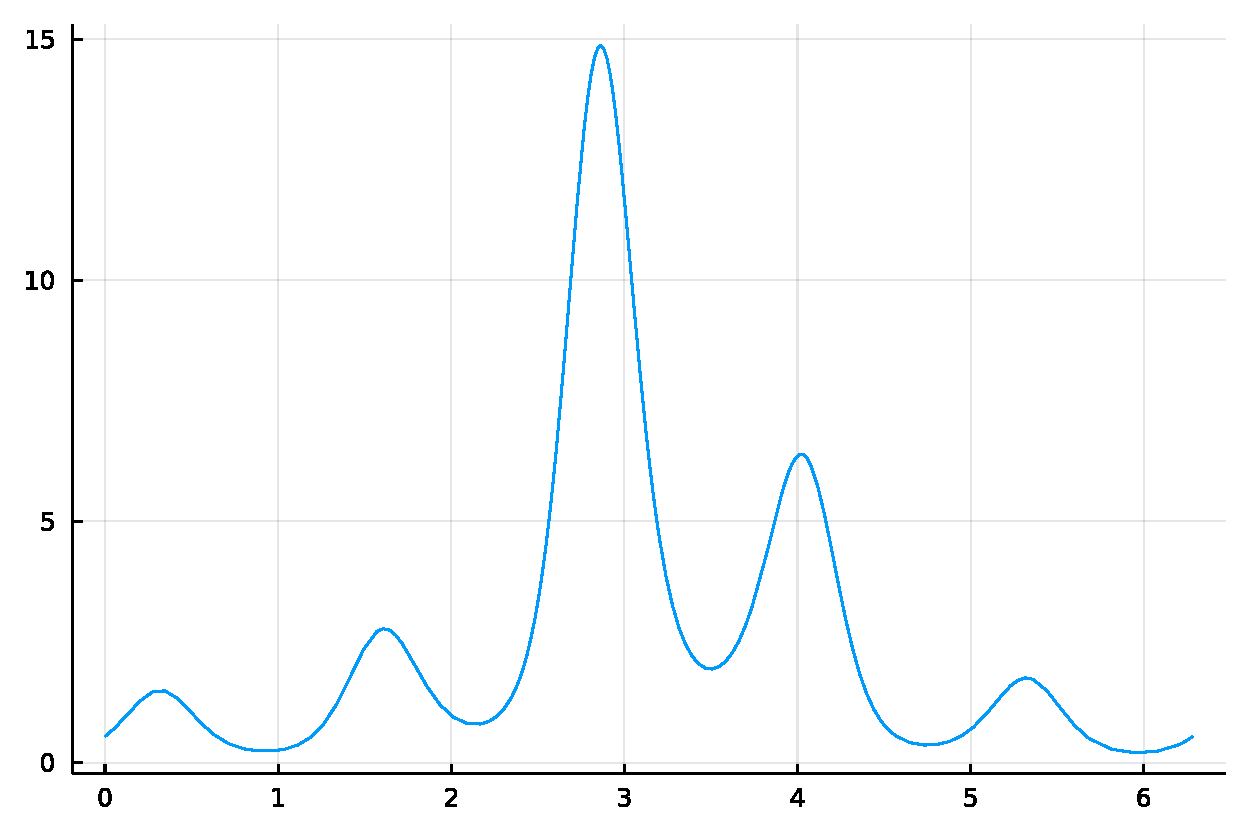
\includegraphics[keepaspectratio,scale = 0.4]{Plot_f(x).pdf}
	\caption{Plot $f(x)$}
\end{figure}

\texttt{ApproxFun.jl}で $f(x)$ を近似してみると、グラフは下のようになる。

\begin{verbatim}
using ApproxFun, FFTW
fc = Fun(f,Laurent())
plot(real(fc))
\end{verbatim}

\begin{figure}[h]
	\centering
	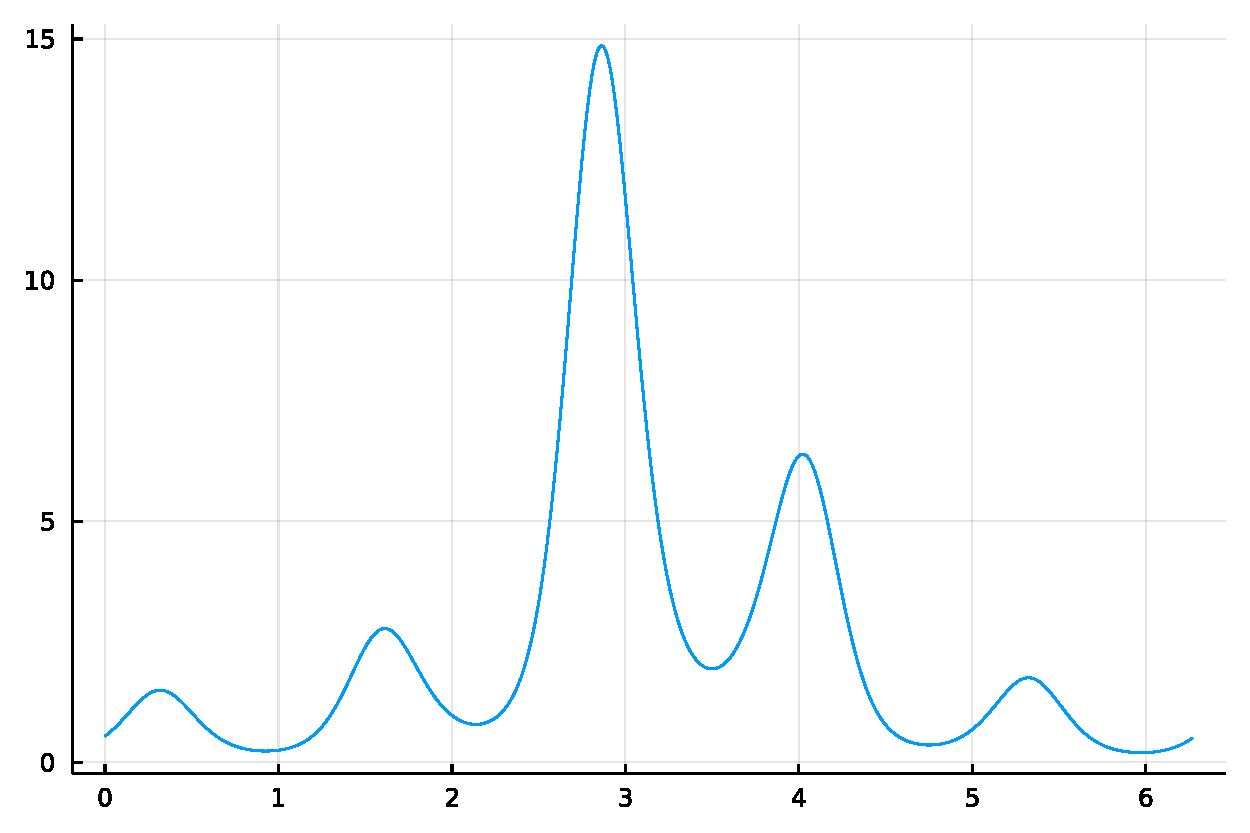
\includegraphics[keepaspectratio,scale = 0.4]{Plot_f(x)_approxfun.pdf}
	\caption{Plot $f(x)$ of \texttt{ApproxFun.jl}}
\end{figure}

フーリエ係数を比較すると一致することが確認できる。

\footnotesize
\begin{verbatim}
m = ncoefficients(fc)
M = Int((m+1)/2)
c = coefficients(fc) # coefficients of ApproxFun
function index_shift(c) # convert c -> fourier coeffs
    return [reverse(c[2:2:end]);c[1:2:end]]
end
a = fouriercoeffs(f,M) 
plot(abs.(a),yscale=:log10,label="computed via FFT")
plot!(abs.(index_shift(c)),yscale=:log10,label = "ApproxFun")
\end{verbatim}
\normalsize

\begin{figure}[h]
	\centering
	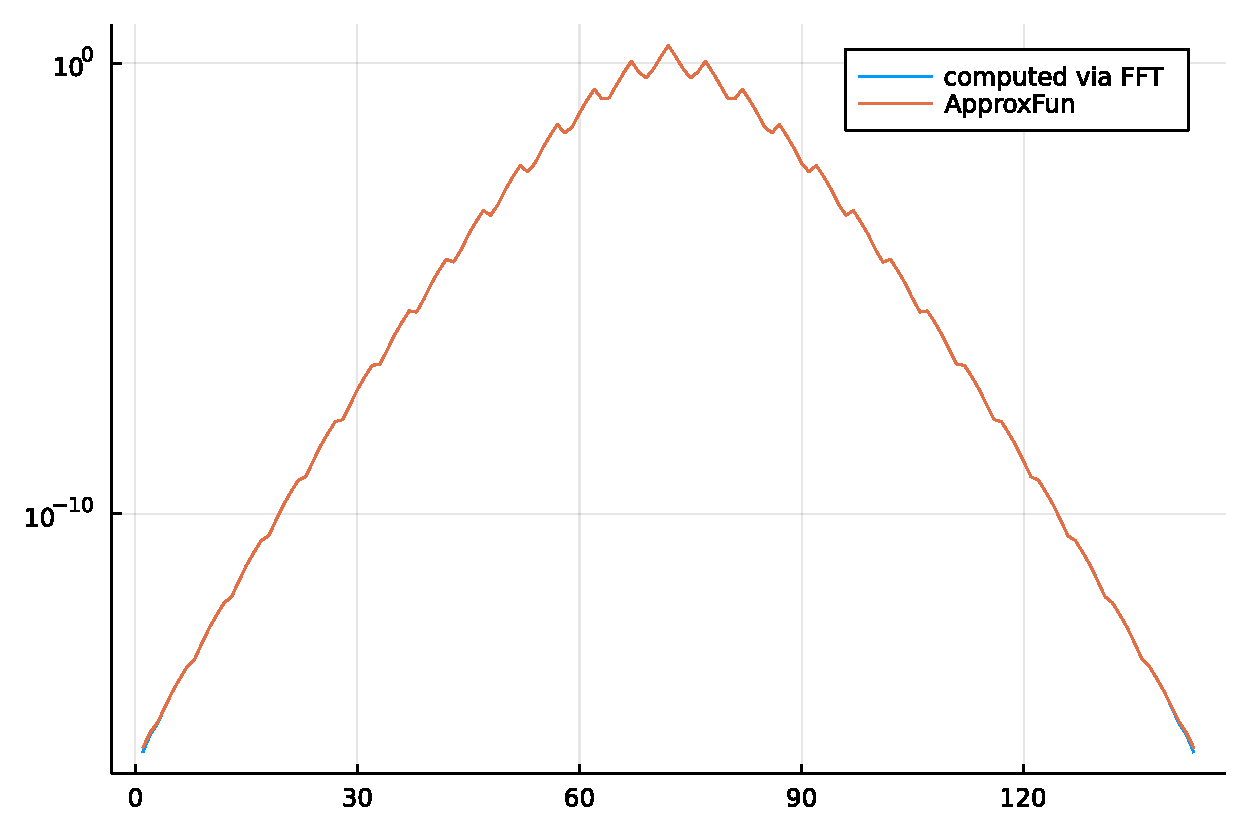
\includegraphics[keepaspectratio,scale = 0.4]{compare_coeffs_FFT_approxfun.pdf}
	\caption{coefficients of FFT and \texttt{ApproxFun.jl}}
\end{figure}

この周期関数の2乗をする場合の畳み込みについて考えてみよう。2乗した関数の概形は、

\begin{verbatim}
plot(real(fc)^2)
\end{verbatim}

\begin{figure}[h]
	\centering
	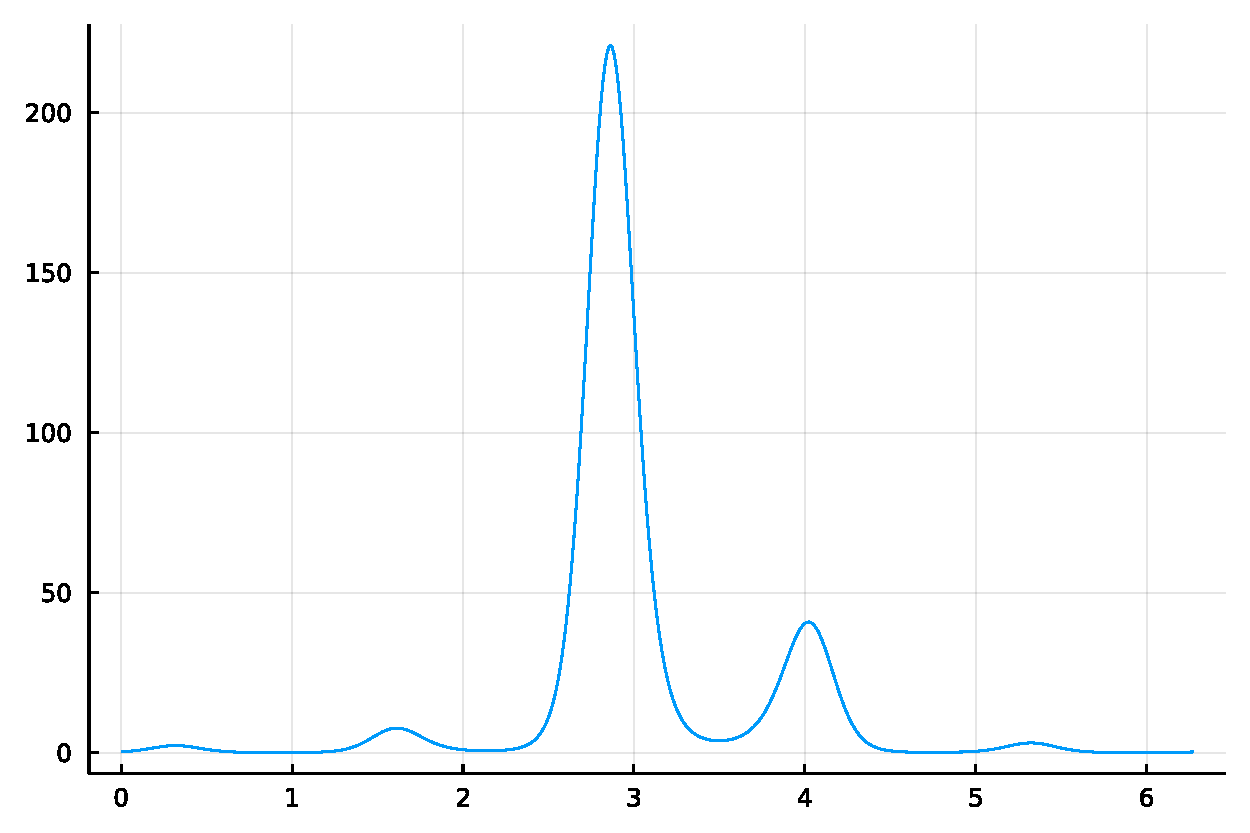
\includegraphics[keepaspectratio,scale = 0.4]{Plot_f(x)^2.pdf}
	\caption{Plot $f(x)^2$}
\end{figure}

一方、FFTアルゴリズムを用いて2乗した関数のフーリエ係数を求め、得たフーリエ級数の概形をプロットすると次のようになる。

\footnotesize
\begin{verbatim}
# FFT Algorithm
p = 2
N = (p-1)*M
ta = [zeros(N,1);a;zeros(N,1)] # 1. Padding zeros
tb = ifft(ifftshift(ta)) # 2. IFFT of ta
tb^p = tb.^p # 3. tb*^tb

# 4. FFT of tb2 
c^p = fftshift(fft(tb^p))*(2.0*p*M-1)^(p-1) 

plot_fourier!(c^p)
\end{verbatim}
\normalsize

\begin{figure}[h]
	\centering
	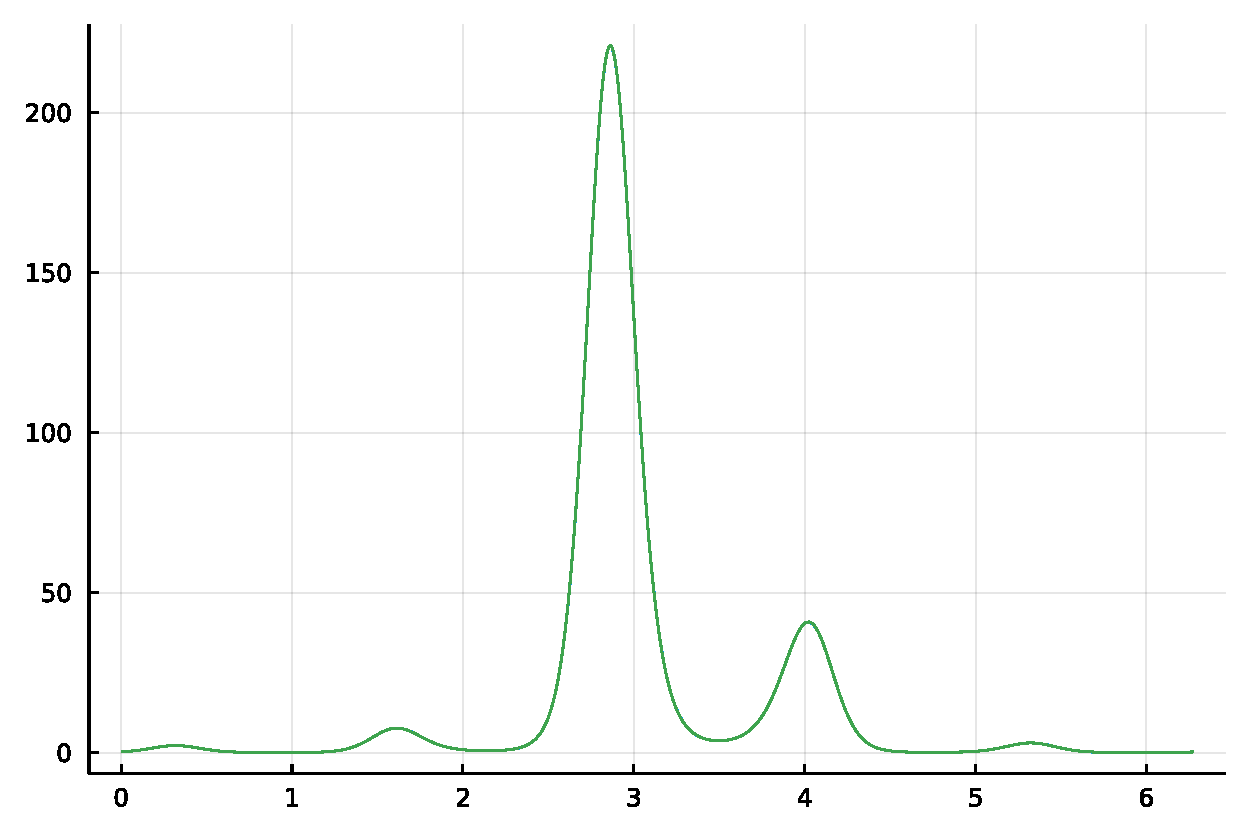
\includegraphics[keepaspectratio,scale = 0.4]{Plot_f(x)_FFT.pdf}
	\caption{Plot $f(x)^2$ and $f(x)^2$ of FFT}
\end{figure}

二つの概形が一致しているのが分かる(水色と赤の曲線がほぼ一致している)。次に、このプログラムを関数化してみよう。

関数が与えられたら、そのフーリエ係数を計算する\texttt{fouriercoeffs}を使って得たフーリエ係数の離散畳み込み(\texttt{powerconvfourier})を計算することで、関数の冪乗を計算できる。
\end{comment}
%---------------------------------------------------------------

\begin{comment}
下記のコードが離散畳み込みを実装した関数になる。また、本論文に記載されているコードは、2段組の都合上、適宜改行されている。

\footnotesize
\begin{verbatim}
function powerconvfourier(a::Vector{Complex{T}}
                                     ,p) where T
    M = Int((length(a)+1)/2)
    N = (p-1)*M

    # 1. Padding zeros: size(ta) = 2pM-1
    ta = [zeros(N,1);a;zeros(N,1)] 

    # 2. IFFT of ta
    tb = ifft(ifftshift(ta)) 
    tb^p = tb.^p # 3. tb*^tb
    c^p = fftshift(fft(tb^p))*(2.0*p*M-1)^(p-1)

    # return (truncated, full) version
    return c^p[N+1:end-N], c^p[p:end-(p-1)]
end
\end{verbatim}
\normalsize

\subsection{離散畳み込みの精度保証付き数値計算}
離散畳み込みの精度保証を行う。離散畳み込みのアルゴリズムには、FFTが含まれるため、まず、FFTの精度保証を行うための関数を定義する。コードについては付録に記載する。
\end{comment}

%---------------------------------------------------------------
\begin{comment}
\begin{verbatim}
M = 150
p = 2
f(x) = erf(sin(3x)+cos(2x))^4
g(x) = f(x)^p

a = fouriercoeffs(f,M) # size(a) = 2M-1
# plot(abs.(a),yscale=:log10,)

ia = map(Interval, a)

length_ia = 2M-1
length_ia_ext = nextpow(2,length_ia)
n = Int((length_ia_ext - length_ia + 1)/2) # 2n-1
ia_ext = map(Interval,im*zeros(length_ia_ext))
ia_ext[n+1:end-n+1] = ia
verifyfft(ia_ext,1)# sign = 1(fft), -1(ifft)
\end{verbatim}
\end{comment}
%---------------------------------------------------------------

\begin{comment}

\texttt{verifyfft}は、要素数が2のべき乗の場合しか実行できないので、step1のpaddingの部分で要素数を調整する。
\begin{align*}
\tilde{a}=(&\underbrace{0, \cdots , 0}_{L\text{個}},\underbrace{0, \cdots , 0}_{N=(p-1)M\text{個}}, \underbrace{a_{-M+1}, \cdots , a_{M-1}}_{2M-1\text{個}}, \\
&\underbrace{0, \cdots , 0}_{N\text{個}},\underbrace{0, \cdots , 0}_{L-1\text{個}}) \in \mathbb{C}^{2pM-2+2L}
\end{align*}

\begin{align*}
c=(&\underbrace{0, \cdots , 0}_{L\text{個}},\underbrace{0, \cdots , 0}_{(p-1)\text{個}}, \underbrace{a_{-p(M-1)}, \cdots , a_{p(M-1)}}_{2p(M-1)+1\text{個}},\\
&\underbrace{0, \cdots , 0}_{(p-1)\text{個}},\underbrace{0, \cdots , 0}_{L-1\text{個}}) \in \mathbb{C}^{2pM-2+2L}
\end{align*}

%step1の \texttt{ia\_ext} が上の $\tilde{a}$ を指し、\texttt{ic\_ext} が $c$ である。2のべき乗になるようにpaddingした分、関数の最後に取り出す値の範囲に注意する。
下記のコードは、区間演算とベクトル、両方の型に対応できるように、多重ディスパッチを利用する離散畳み込みの関数である。

\footnotesize
\begin{verbatim}
function powerconvfourier(a::Vector{Complex{Interval{T}}}
                                     ,p) where T
    M = Int((length(a)+1)/2) # length(a) = 2M-1
    N = (p-1)*M
    ia = map(Interval, a)

    length_ia = 2*p*M-1
    length_ia_ext = nextpow(2,length_ia)# 2pM-2+2L
    
    L = Int((length_ia_ext - length_ia + 1)/2)
    
    # step.1 : padding (p-1)M + L zeros for each sides
    ia_ext = map(Complex{Interval},zeros(length_ia_ext))
    ia_ext[L+N+1:end-L-N+1] = ia  #\tilda{a}

    # step.2 : inverse fft
    #sign = -1 : ifft
    ib_ext = verifyfft(ifftshift(ia_ext), -1) 
    
    # step.3 : power p elementwisely
    ib_ext^p = ib_ext.^p
    
    # step.4 : fft with rescaling
    #sign = 1 : fft
    ic_ext^p = fftshift(verifyfft(ib_ext^p, 1)) 
                  * length_ia_ext^(p-1)  
    
    # return ic_ext^p,ic_ext^p
    # return (truncated, full) version
    return ic_ext^p[L+N+1:end-N-L+1]
                         , ic_ext^p[L+p:end-(L+p-2)] 
end
\end{verbatim}
\normalsize
\end{comment}

%---------------------------------------------------------------
\begin{comment}
\begin{verbatim}
c,c_full = powerconvfourier(a,2);
ic,ic_full = powerconvfourier(ia,2);# 多重ディスパッチ
\end{verbatim}

区間演算は、数値計算で得た値の範囲全体を含むため、\texttt{ic\_full $\in$ c\_full}が成り立つ。

また、下の図からテイルに$10^{-15}$ほどの誤差が含まれていることがわかる。

\begin{verbatim}
using IntervalArithmetic:mid
@show c_full .∈ ic_full
plot(abs.(c_full),yscale=:log10,label="non-rigorous")
plot!(mid.(abs.(ic_full)),yscale=:log10,label="rigorous")
\end{verbatim}
\end{comment}
%---------------------------------------------------------------

%\end{document}